\documentclass{article}
\usepackage[T1]{fontenc}
\usepackage{lmodern}
\usepackage{graphicx}
\usepackage{amsmath,amssymb}
\usepackage[a4paper,margin=2cm]{geometry}
\usepackage[absolute,overlay]{textpos}
\setlength{\TPHorizModule}{1mm}
\setlength{\TPVertModule}{1mm}
\usepackage[indonesian]{babel}
\usepackage{hyperref}
\setlength{\emergencystretch}{2em}
% unit: Halaman 26

\begin{document}

% === Halaman 26 (python/native) ===

Inversi Permutasi (IP-1)

• Permutasi terakhir dilakukan setelah 16 kali putaran

   terhadap gabungan  blok kiri dan blok kanan. 

• Permutasi menggunakan matriks permutasi awal 

balikan (IP-1 ) sbb:

40 

8 

48 

16 

56 

24 

64 

32 

39 

7 

47 

15 

55 

23 

63 

31 

38 

6 

46 

14 

54 

22 

62 

30 

37 

5 

45 

13 

53 

21 

61 

29 

36 

4 

44 

12 

52 

20 

60 

28 

35 

3 

43 

11 

51 

19 

59 

27 

34 

2 

42 

10 

50 

18 

58 

26 

33 

1 

41 

9 

49 

17 

57 

25 


26

% deskripsi: gambar native xref 60
\noindent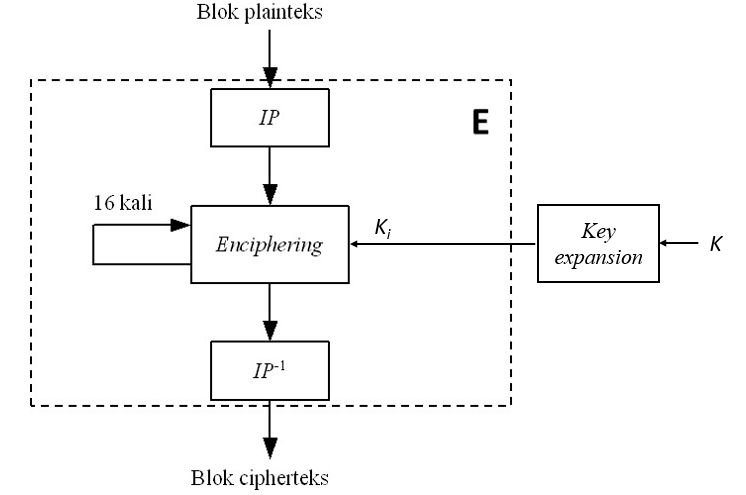
\includegraphics[width=0.85\textwidth]{../../images/python/page_026_img_01.png}

\end{document}
